\documentclass{article}
\usepackage{v-equation}
\vgeometry

\begin{document}
\def\gdrive{https://drive.google.com/drive/folders/1_FtjXAUlK_I72Fzq060RD8MxSyqj788g?usp=share_link}

\vtitle[Coulomb’s Law]
\begin{center}
\begin{tikzpicture}
[thick]
\tzcoor*(3.5,  3)(Q2){$q_2$}[br](4pt)
\tzcoor*(1,  2)(Q1){$q_1$}[a](4pt)
\tzcoor*(0,  0)(O){$O$}[br]
	\tzaxes(-0.5, -0.5)(5,4){$x$}{$y$}
	\tzline[->](O)(Q1){$\vec{r}_1$}[ml]
	\tzline[->](O)(Q2){$\vec{r}_2$}[mb]
	\tzline[->](Q1)(Q2){$\vec{r}_{21}$}[ma]
	\tzline[->](Q2)($(Q1)!1.65!(Q2)$){$\vec{F}_{21}$}[r]
\end{tikzpicture}
\end{center}
\vspace*{\fill}
\begin{align*}
\vec{F}_{21} &= \dfrac{1}{4\pi\epsilon_0} \dfrac{q_1q_2}{\left| \vec{r}_2-\vec{r}_1  \right|^3} \left( \vec{r}_2 - \vec{r}_1 \right)\\[5 mm]
\vec{F}_{12} &= \dfrac{1}{4\pi\epsilon_0} \dfrac{q_1q_2}{\left| \vec{r}_1-\vec{r}_2  \right|^3} \left( \vec{r}_1 - \vec{r}_2 \right)
\end{align*}
\vspace*{\fill}
\pagebreak

\vspace*{\fill}
\begin{align*}
\vec{F}_{21} &= \dfrac{1}{4\pi\epsilon_0} \dfrac{q_1q_2}{\left| \vec{r}_{21} \right|^2} \left( \hat{r}_{21} \right)\\[5 mm]
\vec{F}_{21} &= \dfrac{1}{4\pi\epsilon_0} \dfrac{q_1q_2}{\left| \vec{r}_{2} -\vec{r}_1 \right|^2} \left( \dfrac{\vec{r}_{21}}{\left| \vec{r}_{21}\right|} \right)\\[5 mm]
\vec{F}_{21} &= \dfrac{1}{4\pi\epsilon_0} \dfrac{q_1q_2}{\left| \vec{r}_{2} -\vec{r}_1 \right|^2} \left( \dfrac{\vec{r}_2 -\vec{r}_1}{\left| \vec{r}_2 - \vec{r}_1\right|} \right)\\[5 mm]
\vec{F}_{21} &= \dfrac{1}{4\pi\epsilon_0} \dfrac{q_1q_2}{\left| \vec{r}_2-\vec{r}_1  \right|^3} \left( \vec{r}_2 - \vec{r}_1 \right)
\end{align*}
\vspace*{\fill}
\pagebreak

\vspace*{\fill}
\begin{center}
	\fbox{\qrcode[height=2cm]{\gdrive}}
\end{center}
\vspace*{\fill}
\end{document}
